% !TEX root = ../main.tex
\begin{figure}[htbp]
\centering
\begin{minipage}[c]{.55\linewidth}
\centering
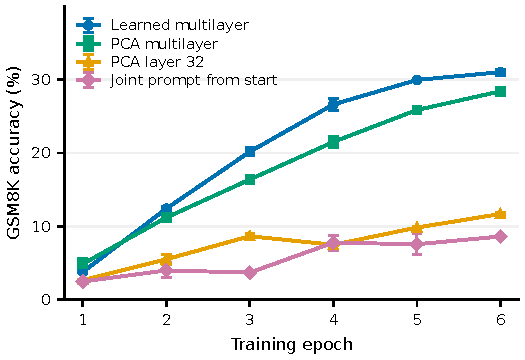
\includegraphics[width=\linewidth]{figures/representation_shared2_sd.pdf}
\end{minipage}\hfill
\begin{minipage}[c]{.43\linewidth}
\centering
% !TEX root = ../main.tex
% Generated from exact per-seed counts; parentheses are sample SD, ddof=1.
\begingroup
\small
\setlength{\tabcolsep}{3pt}
\renewcommand{\arraystretch}{1.25}
\begin{tabular}{@{}lr@{}}
\toprule
Variant & Accuracy (\%) \\
\midrule
Learned, 16/24/32 & \textbf{30.76} {\scriptsize (0.39)} \\
PCA, 16/24/32 & 28.43 {\scriptsize (0.19)} \\
PCA, layer 32 & 11.20 {\scriptsize (0.56)} \\
Epoch 0 learned prompt encoder & 8.70 {\scriptsize (0.33)} \\
\bottomrule
\end{tabular}
\endgroup

\end{minipage}
\caption{\textbf{Representation and conditioning choices change reasoning performance.} ELF-B on GSM8K with shared $t=\tau^2$, 32 steps, and ELF EMA $0.999$. \textbf{Left:} learning curves over seeds 42/123 (bars: seed SD). \textbf{Right:} epoch-six means over seeds 42/123/456/789 (parentheses: seed SD); reporting conventions are in Appendix~\ref{app:experimentdetails}. All latents are whitened and 1,024-dimensional. The first three variants use frozen Qwen prompt activations. The fourth uses learned multilayer answer latents and a randomly initialized prompt encoder trained jointly from epoch zero (prompt EMA $0.999$). The epoch-six ordering persists with the identity clock $t=\tau$ (Appendix~\ref{app:representationclock}).}
\label{fig:representationcomparison}
\end{figure}
